\documentclass[aps,prd,onecolumn,superscriptaddress,nofootinbib]{revtex4-2}

% — Packages —
\usepackage[utf8]{inputenc}
\usepackage[T1]{fontenc}
\usepackage{lmodern}
\usepackage{amsmath,amssymb,bm,mathtools,amsthm}
\usepackage{graphicx}
\usepackage{adjustbox}
\usepackage{xcolor}
\usepackage{microtype}
\usepackage[unicode, pdfencoding=auto, psdextra]{hyperref}
\usepackage{enumitem}
\usepackage{tikz}
\usepackage{booktabs}
\usepackage{siunitx}
\sisetup{detect-all}
\usetikzlibrary{arrows.meta,positioning,fit,calc,shapes.geometric,shapes.multipart,backgrounds}

% — Colors for flowchart —
\definecolor{flowBlue}{HTML}{1F77B4}
\definecolor{flowPurple}{HTML}{9467BD}
\definecolor{flowGreen}{HTML}{2CA02C}
\definecolor{flowOrange}{HTML}{FF7F0E}
\definecolor{flowRed}{HTML}{D62728}
\definecolor{flowGray}{HTML}{7F7F7F}

% — Hyperref —
\hypersetup{
  colorlinks=true,
  linkcolor=blue,
  citecolor=blue,
  urlcolor=blue
}

% — PDF string sanitization —
\pdfstringdefDisableCommands{%
  \def\OmL{OmegaLambda}%
  \def\Omm{Omega m0}%
  \def\cgeo{cgeo}%
  \def\alphaM{alphaM}%
  \def\eps{epsilon}%
  \def\boxed#1{#1}%
  \def\mu{mu}%
  \def\alpha{alpha}%
  \def\alpha_M{alphaM}%
  \def\Omega_\Lambda{OmegaLambda}%
}

% — Math tweaks —
\allowdisplaybreaks

% — Macros —
\providecommand{\mpl}{M_{\rm P}}
\providecommand{\OmL}{\Omega_\Lambda}
\providecommand{\Omm}{\Omega_{m0}}
\providecommand{\cgeo}{c_{\rm geo}}
\providecommand{\alphaM}{\alpha_M}
\providecommand{\eps}{\varepsilon}
\providecommand{\be}{\begin{equation}}
\providecommand{\ee}{\end{equation}}
\providecommand{\bse}{\begin{subequations}}
\providecommand{\ese}{\end{subequations}}

% — Theorem-like environments —
\newtheorem{definition}{Definition}
\newtheorem{hypothesis}{Hypothesis}
\newtheorem{lemma}{Lemma}
\newtheorem{proposition}{Proposition}
\newtheorem{theorem}{Theorem}
\newtheorem{corollary}{Corollary}

\begin{document}

\title{Modular Response in Free Quantum Fields:\\
A KMS/FDT Theorem and Conditional Extensions}

\author{[Authors]}
\affiliation{[Institutions]}
\date{}

\begin{abstract}
\textbf{Part I (Theoremic core, free/Gaussian Hadamard QFT).} We prove that, for small causal diamonds (CHM) in locally Hadamard states on globally hyperbolic spacetimes and within a safe window \(\epsilon_{\rm UV}\ll\ell\ll \min\{L_{\rm curv},\lambda_{\rm mfp},m_i^{-1}\}\), the MI/moment-kill projector isolates a finite \(\ell^4\) modular response with coefficient equal to its flat-space value, the projected KMS/FDT susceptibility is positive, and coarse-graining over the wedge family produces a universal weak-field prefactor \(5/12=(4/3)\times(5/16)\). The fractional KMS defect between CHM diamonds and half-spaces scales as \(\mathcal O((\ell/L_{\rm curv})^2)+\mathcal O((\ell H)^2)\). The QFT sensitivity is \(\beta=2\pi C_T I_{00}=0.02086\pm 0.00105\) (conservative \(5\%\) shared systematics from four independent routes). A scheme-invariant background normalization yields \(\OmL=\beta\, f\,\cgeo\).

\smallskip
\textbf{Part II (Conditional extensions).} We separate \emph{definition} (flat-space \(\eps\) from modular response) from \emph{mapping} (constitutive identification \(\delta\ln M^2=\beta\,\delta\eps\)), keep the distance sector GR-like (\(\alpha_M\simeq 0\)), and obtain weak-field growth \(\mu(\eps)=1/(1+\tfrac{5}{12}\eps)\). The entropy-driven law \(d\eps/d\ln a\ge 0\) follows from KMS/FDT positivity with a fixed ``budget" \(\int \eps\,d\ln a=\OmL\). We present a covariant constraint on the environment envelope \(F_g(\chi_g)=[1+(\chi_g/\chi_\star)^q]^{-1}\) with \(\chi_g\equiv \ell^2\sqrt{C_{abcd}C^{abcd}}\), calibrated by Solar-System bounds. Cosmological illustrations (an \(S_8\) band and \(H_0\) shifts) are \textbf{toy/illustrative}, conditional on extension to interacting QFTs and the covariant KMS\(\to\)FRW link; all values propagate the \(\pm5\%\) \(\beta\) uncertainty.

\smallskip
\emph{What is new.} (i) Completed proofs in the Gaussian/Hadamard sector, including a covariant KMS\(\to\)FRW averaging lemma with explicit error budget; (ii) \textbf{stated assumptions for Lemma C (relative entropy \(\leftrightarrow\) canonical energy in the projected diamond) and Lemma D (uniqueness of \(M^2\) coupling at working order) in interacting QFTs, pending rigorous proof}; (iii) semi-analytic quantification of the safe-window volume fraction \(f_V(\ell_{\min})\) with Press--Schechter/Sheth--Tormen inputs; (iv) a symmetry-constrained \(F_g\) envelope with calibrated \(\chi_\star\) and \(q\); (v) uncertainty propagation of \(\beta\) into \(S_8\) and \(H_0\) bounds. Part II remains explicitly labeled as conditional.

\smallskip
\emph{Caveat.} Part II relies on unproven extensions to interacting QFTs, which may fail pending further theoretical development; we label these elements explicitly and provide a roadmap to rigor.
\end{abstract}

\maketitle

% ============================================================
\section*{Reader’s map: Part I (Theorem) vs.\ Part II (Conditional)}
\noindent \textbf{Part I (Secs.~\ref{sec:scope}–\ref{sec:five-twelve}, Apps.~\ref{app:MI}–\ref{app:chm-kms-estimate}):} proven results for free/Gaussian Hadamard fields at working order.\\
\textbf{Part II (Secs.~\ref{sec:def-vs-map}–\ref{sec:data}, Apps.~\ref{app:fv}, \ref{app:microlocal}, \ref{app:numerics}):} conditional extensions, \emph{assumptions} C \& D (pending proof), safe-window fraction, KMS\(\to\)FRW link, symmetry envelope, and toy/illustrative numerics (App.~\ref{app:numerics}) with propagated uncertainties.

% ===============================
\section{Scope, Working Order, and Safe-Window Quantification (Part I)}
\label{sec:scope}

\paragraph{Working order and state class.} We work to \(\mathcal O(\ell^4)\) in the MI/moment-kill projector channel, treating curvature/contact terms as \(\mathcal O(\ell^6)\). States are locally Hadamard.

\paragraph{KMS applicability (CHM diamonds).} Exact BW KMS holds for half-spaces; CHM diamonds inherit it with fractional defect \(\mathcal O((\ell/L_{\rm curv})^2)+\mathcal O((\ell H)^2)\) (App.~\ref{app:chm-kms-estimate}).

\paragraph{Safe-window volume fraction.} Define a conservative admissible scale
\be
\ell_{\max}(x)\equiv \zeta\;\min\Big\{L_{\rm curv}(x),\ \lambda_{\rm mfp}(x),\ m_i^{-1}(x)\Big\},\qquad \zeta=0.1.
\ee
Using Press--Schechter/Sheth--Tormen mass functions and NFW curvature proxies \(L_{\rm curv}^{-2}\sim (R_{abcd}R^{abcd})^{1/2}\) with substructure excision parameter \(\xi\), we estimate the comoving volume fraction \(f_V(\ell_{\min})=\mathrm{Vol}\{x:\,\ell_{\max}(x)>\ell_{\min}\}/\mathrm{Vol}_{\rm tot}\). A semi-analytic survey (App.~\ref{app:fv}) shows voids dominate \(f_V\), while dense cores lack a window; representative values at \(z\!\sim\!0\) for \(\ell_{\min}\in[1,100]\) pc are \(f_V\sim 0.6{-}0.95\) for \(\xi\in[0.2,0.5]\). This enters only as a domain-of-validity indicator. A parameter sensitivity sweep (varying \(\zeta,\ \lambda_{\rm mfp},\ \xi\)) yields more conservative fractions \(f_V\sim 0.4{-}0.7\) (App.~\ref{app:fv}), addressing potential over-optimism in structured regions.

\paragraph{Angle invariance as a null test.} The continuous-angle product \(\mathcal C_\Omega=f(\theta)\,\cgeo(\theta)\) is analytic and \(\theta\)-independent; residuals are shown as a null check, not a precision claim.

% ===============================
\section{A2–KMS Theorem (Gaussian/Hadamard Sector)}
\label{sec:theorem}

\begin{theorem}[Projected modular response and positivity]
Let \(\mathcal Q\) be a free (Gaussian) QFT on a globally hyperbolic spacetime and \(\rho\) a locally Hadamard state. For a causal diamond of radius \(\ell\) with \(\ell\ll L_{\rm curv}\) and the MI/moment-kill projector that cancels \(r^0\) and \(r^2\) moments, the MI-subtracted modular response obeys
\be
\delta\!\langle K_{\rm sub}\rangle=(2\pi C_T I_{00})\,\ell^4\,\delta\eps+\mathcal O(\ell^6),
\ee
with coefficient equal to the flat-space value. The retarded susceptibility \(\chi_{QK}\) in the projected channel is positive (FDT), and wedge averaging yields the universal weak-field prefactor \(5/12\). The fractional deviation from BW KMS is \(\mathcal O((\ell/L_{\rm curv})^2)+\mathcal O((\ell H)^2)\).
\end{theorem}

\noindent\emph{Proof.} Hadamard microlocal expansions reduce all UV data to the Minkowski parametrix; MI/moment-kill cancels local counterterms to \(\mathcal O(\ell^4)\) (App.~\ref{app:MI}). BW KMS fixes linear-response normalization and sign; positivity follows from the Bogoliubov--Kubo--Mori metric. Isotropic contraction and CHM segment ratio yield \(5/12\) (Sec.~\ref{sec:five-twelve}). CHM vs.\ half-space defects scale as stated in Riemann-normal coordinates (App.~\ref{app:chm-kms-estimate}). \qed

\begin{corollary}[Background zero mode]
The FRW zero mode satisfies the scheme-invariant normalization
\(\OmL=\beta\,f\,\cgeo\), with \(\beta=2\pi C_T I_{00}\).
\end{corollary}

% ===============================
\section{QFT Input: \texorpdfstring{$\beta=2\pi C_T I_{00}$}{beta} and Error Budget}
\label{sec:beta}
We evaluate \(\beta\) via four independent routes: (a) real-space CHM; (b) spectral/Bessel; (c) Euclidean time-slicing; (d) replica finite-difference. The spread is \(\lesssim 1\%\). We adopt a conservative
\be
\beta=0.02086\pm 0.00105 \quad (5\%~\text{shared systematics}).
\ee
Angle invariance is used as a null residual test.

% ===============================
\section{Weak-Field Prefactor \texorpdfstring{$5/12$}{5/12}}
\label{sec:five-twelve}
The isotropic BW channel gives \(\langle T_{kk}\rangle=(1+w)\rho\) with UV \(w=1/3\Rightarrow 4/3\). Averaging over CHM segments yields \(5/16\), so \(5/12=(4/3)\times(5/16)\). Details in App.~\ref{app:five-twelve}.

% ============================================================
\section{Definition vs.\ Mapping (Part II; Conditional)}
\label{sec:def-vs-map}

\paragraph{Definition (flat-space QFT).}
\be
\delta\!\langle K_{\rm sub}(\ell)\rangle=\underbrace{(2\pi C_T I_{00})}_{\beta}\,\ell^4\,\delta\eps(x)+\mathcal O(\ell^6).
\label{eq:eps-def}
\ee

\paragraph{Mapping (constitutive; distances GR-like).}
In the c\(_T\!=\!1\), \(\alpha_B\!=\!0\) EFT corner with isotropy, we \emph{identify} at working order
\be
\delta\ln M^2=\beta\,\delta\eps,\qquad
\mu(\eps)=\frac{1}{1+\tfrac{5}{12}\,\eps},\qquad \alpha_M\simeq 0~\text{in distances}.
\label{eq:mapping}
\ee
This is a \textbf{constitutive closure}, not a derived macroscopic law; it is falsified by log-\(\ell\) residuals, \(|d_L^{\rm GW}/d_L^{\rm EM}-1|>5\times 10^{-3}\), or \(\OmL\) inconsistent with \(\beta f\cgeo\).

% ===============================
\section{Covariant KMS \texorpdfstring{$\to$}{->} FRW Link and Error Control}
\label{sec:kms-frw}
Let \(s\) denote modular time with \(\beta_{\rm KMS}=2\pi/\kappa\) locally. Averaging the retarded kernel over a comoving congruence of diamonds and reparametrizing \(s\mapsto \ln a\) induces the FRW background factor \(f\,\cgeo\); diffeomorphism covariance is preserved because the averaging functional depends only on local curvature scalars and the diamond foliation. The total fractional defect in the kernel obeys
\be
\frac{\delta\chi}{\chi_{\rm BW}}=\mathcal O\!\Big((\ell/L_{\rm curv})^2\Big)+\mathcal O\!\big((\ell H)^2\big),
\ee
which is negligible for \(\ell\!\sim\!10\,\mathrm{pc}\), \(L_{\rm curv}\!\sim\!10\,\mathrm{Mpc}\), \(H^{-1}\!\sim\!4\,\mathrm{Gpc}\).

\emph{Analyticity caveat.} The reparametrization \(s\to\ln a\) is conjectured to preserve KMS analyticity for the averaged kernel by matching modular flow to the FRW scale factor; a rigorous proof of the averaged kernel’s analytic properties remains open and likely requires a spectral/microlocal treatment (see e.g.\ Hollands \& Wald 2001). We list this as a priority item in Sec.~\ref{sec:path}.

% ===============================
\section{Assumptions for Interacting Extensions at Working Order (Part II)}
\label{sec:assumptions}

\subsection{Assumption C: Relative entropy \texorpdfstring{$\leftrightarrow$}{<->} canonical energy in the projected diamond}
\label{sec:lemmaC}

\begin{hypothesis}[Assumption C]
For a local algebra \(\mathcal A(B_\ell)\) of an interacting Hadamard QFT obeying the microlocal spectrum condition and time-slice axiom, let \(\sigma\) be the reference diamond state (vacuum-equivalent at short distance) with modular operator \(\Delta_\sigma\) and modular Hamiltonian \(K_\sigma\). For a smooth one-parameter family \(\rho(\lambda)\) with \(\rho(0)=\sigma\) and \(\dot\rho\equiv \partial_\lambda\rho|_0\), the MI/moment-kill projected second variation of Araki relative entropy equals the canonical energy quadratic form of the projected stress tensor, up to \(\mathcal O(\ell^6)\) remainders:
\be
\left.\frac{d^2}{d\lambda^2}\right|_0 S(\rho(\lambda)\Vert\sigma)
=\mathcal E_{\rm can}^{\rm proj}[\delta T;\,\xi_{\rm CHM}]
=\iint \chi_{QK}^{\rm proj}(x,x')\,\delta Q(x)\,\delta K_{\rm sub}(x')\,d^4x\,d^4x' \ge 0,
\ee
with \(\chi_{QK}^{\rm proj}\) positive-definite. The equality is \emph{assumed} to hold for interacting QFTs at working order \(\mathcal O(\ell^4)\).
\end{hypothesis}

\noindent\emph{Rationale and status (sketch).}
(i) \textbf{Second variation as BKM metric.} For type III\(_1\) local algebras, Araki relative entropy is well-defined; near \(\sigma\), the second variation equals the Bogoliubov--Kubo--Mori (quantum Fisher) metric evaluated on the tangent vector generated by \(\delta K_\sigma\).\\
(ii) \textbf{Projector isolation (assumed).} We assume the MI/moment-kill projector cancels contact terms and the \(r^0,r^2\) moments built from Hadamard \(v,w\) coefficients through \(\mathcal O(\ell^4)\) in interacting Hadamard QFTs, leaving the flat-space coefficient; a full microlocal proof of stability under interactions is outstanding (cf.\ Hollands \& Wald 2001).\\
(iii) \textbf{Ward/canonical energy link.} Using diffeomorphism Ward identities and the time-slice axiom, the BKM quadratic form for stress-generated deformations integrates to the canonical energy associated with \(\xi_{\rm CHM}\); projecting both sources yields \(\mathcal E_{\rm can}^{\rm proj}\).\\
(iv) \textbf{Boundary terms and positivity.} Boundary contributions vanish under the MI/moment-kill projector; this is consistent with quantum energy inequality techniques (Fewster \& Hollands). Positivity is expected from KMS/BKM positivity in the projected channel. A complete derivation remains future work (Sec.~\ref{sec:path}).

\subsection{Assumption D: Uniqueness of the \texorpdfstring{$M^2$}{M^2} coupling at working order}
\label{sec:lemmaD}

\begin{hypothesis}[Assumption D]
In the c\(_T\!=\!1\), \(\alpha_B\!=\!0\) EFT corner linearized about FRW, with isotropy, parity, and time-reversal, the only background scalar coupling that survives the MI/moment-kill projection at \(\mathcal O(\ell^4)\) and modifies the weak-field growth sector while keeping distances GR-like is \(\delta\ln M^2\). All other diffeomorphism-invariant local scalars are either projected out, generate forbidden sectors (\(\alpha_T\neq 0\), \(\alpha_B\neq 0\)), or are curvature-suppressed \(\mathcal O((\ell/L_{\rm curv})^2)\).
\end{hypothesis}

\noindent\emph{Rationale and status (sketch).}
Within the \(c_T=1,\ \alpha_B=0\) EFT corner and isotropy, parity, time-reversal, the MI/moment-kill projector removes total derivatives and lower moments, while curvature-built scalars (e.g., \(R,\ \nabla^2R,\ R_{ab}R^{ab}\)) are \(\mathcal O((\ell/L_{\rm curv})^2)\)-suppressed at working order. We therefore \emph{assume} that the only unsuppressed background scalar coupling that modifies weak-field growth while keeping distances GR-like is \(\delta\ln M^2\). A cohomological/Ward-identity proof is outlined in Sec.~\ref{sec:path} and left to future work.

% ===============================
\section{Entropy-Driven \texorpdfstring{$\varepsilon(a)$}{epsilon(a)} and Growth (Conditional)}
\label{sec:epsilon}

\paragraph{KMS/FDT positivity.}
Let \(\hat Q\) be the boost-energy flux and \(\chi_{QK}^{\rm proj}\) the retarded kernel in the projected channel. Then
\be
\frac{d\eps}{d\ln a}=\sigma(a)\,\mathcal I(a),\qquad \sigma(a)\ge 0,\ \ \mathcal I(a)\ge 0,\qquad
\int \eps\,d\ln a=\OmL=\beta\,f\,\cgeo.
\ee

\paragraph{Fixed-point with growth.}
The growth factor \(D(a)\) satisfies
\be
\frac{d^2 D}{d(\ln a)^2}
+\Big(2+\frac{d\ln H}{d\ln a}\Big)\frac{dD}{d\ln a}
-\frac{3}{2}\,\Omega_m(a)\,\mu(\eps(a))\,D=0,\qquad
\mu(\eps)=\frac{1}{1+\tfrac{5}{12}\eps}.
\ee

\paragraph{Variational bounds (extremals).}
Convex-order arguments imply late-loaded \(\eps(a)\) minimizes \(S_8\) and early-loaded maximizes it, under monotonicity and budget. We therefore report an \(S_8\) \emph{band} bracketed by these extremals; any illustrative kernel (e.g., logarithmic exposure) must lie within the band.

% ===============================
\section{Environment Envelope from Symmetry and Calibration}
\label{sec:env}

\paragraph{Covariant envelope.}
We take
\be
F_g(\chi_g)=\frac{1}{1+(\chi_g/\chi_\star)^q},\qquad \chi_g\equiv \ell^2\sqrt{C_{abcd}C^{abcd}},
\ee
with axioms: covariance, equivalence principle, normalization neutrality (no effect in weak curvature), and Solar-System compliance.

\paragraph{Calibration example.}
For a Schwarzschild source, \(\sqrt{C^2}=\sqrt{48}\,GM/r^3\). With \(\ell=10\,\mathrm{pc}\), \(r=1\,\mathrm{AU}\), the Solar value is \(\chi_\odot\simeq \ell^2 \sqrt{48}\,GM_\odot/r^3\approx 2.6\times 10^{22}\). Requiring \(F_g(\chi_\odot)\le \epsilon_{\rm SS}=10^{-5}\) with \(q=2\) yields
\be
\chi_\star \le \chi_\odot\,\epsilon_{\rm SS}^{1/2}\approx 8.2\times 10^{19}.
\ee
Choosing \(\chi_\star=10^{18}\) and \(q=2\) ensures \(\,F_g(\chi_\odot)\lesssim 10^{-9}\) (strong gating in Solar System) while \(F_g\simeq 1\) in galactic/cluster environments (\(\chi_g\ll \chi_\star\)), so cosmological growth is unaffected by the envelope.

\emph{Phenomenology and alternatives.} The choice \(F_g(\chi_g)=[1+(\chi_g/\chi_\star)^q]^{-1}\) with \(q=2\) and \(\chi_g\propto \sqrt{C_{abcd}C^{abcd}}\) is a simple, covariant parameterization that ensures Solar-System suppression. Alternative forms (e.g., \(q=1\), or \(\chi_g\propto R\)) are viable and will be adjudicated by data; our scripts allow these substitutions.

% ===============================
\section{Structural Checks (Algebraic; Not 4D Surrogates)}
\label{sec:substrates}
HQTFIM and Gaussian chains confirm the algebraic ingredients (first-law channel, constant+log trend, vanishing plateau after subtraction, and positivity in the projected kernel). They are \emph{not} curved 4D surrogates.

% ===============================
\section{Proof Program Status and Falsifiers}
\label{sec:program}
\textbf{Lemma A} (diamond KMS control): scaling proven, sharp bounds left to microlocal analysis. \textbf{Lemma B} (projector universality): established. \textbf{Lemma C} and \textbf{Lemma D}: \textbf{stated here as assumptions pending proof} (Secs.~\ref{sec:lemmaC}, \ref{sec:lemmaD}). \textbf{Lemma E} (FDT positivity): follows from BKM positivity. \textbf{Lemma F} (geometric \(5/12\)): derived.\\
\textbf{Falsifiers:} (i) persistent \(\ell^4\log\ell\) residuals in the projector channel; (ii) GW/EM distance ratio beyond \(5\times 10^{-3}\); (iii) \(|\dot G/G|\gtrsim 10^{-12}\,\mathrm{yr}^{-1}\); (iv) \(\OmL\) inconsistent with \(\beta f\cgeo\); (v) \(S_8\) outside the extremal band for all admissible monotone \(\eps(a)\) satisfying the budget; (vi) positivity failure in Assumption C tests.

% ===============================
\section{Path to Rigor for Part II}
\label{sec:path}
We outline key steps to turn the conditional elements of Part II into theorems:
\begin{itemize}[leftmargin=*]
  \item \textbf{Projector stability (interactions).} Prove that the MI/moment-kill projector isolates the \(\ell^4\) term in interacting Hadamard QFTs by establishing stability of Hadamard \(v,w\) under perturbation and explicit \(\mathcal O(\ell^6)\) bounds (cf.\ Hollands \& Wald 2001).
  \item \textbf{KMS\(\to\)FRW analyticity.} Provide a spectral/microlocal proof that the comoving-diamond average preserves KMS analyticity after \(s\mapsto \ln a\), quantifying the defect beyond \(\mathcal O((\ell/L_{\rm curv})^2)+\mathcal O((\ell H)^2)\).
  \item \textbf{Cohomological uniqueness.} Complete a Ward/cohomology derivation that \( \delta\ln M^2\) is the unique scalar coupling at working order in the \(c_T=1,\ \alpha_B=0\) isotropic sector.
  \item \textbf{Envelope constraints.} Derive data-driven bounds on \(F_g\) (including alternatives \(q,\ \chi_g\)) consistent with Solar-System and cosmological growth, replacing phenomenological choices.
  \item \textbf{Domain quantification.} Replace semi-analytic \(f_V\) with simulation-calibrated maps; propagate uncertainties from \(\lambda_{\rm mfp}\) and substructure \(\xi\).
\end{itemize}

% — Vertical, color-coded pipeline figure —
\begin{figure*}[t]
\centering
\begin{adjustbox}{max width=\linewidth}
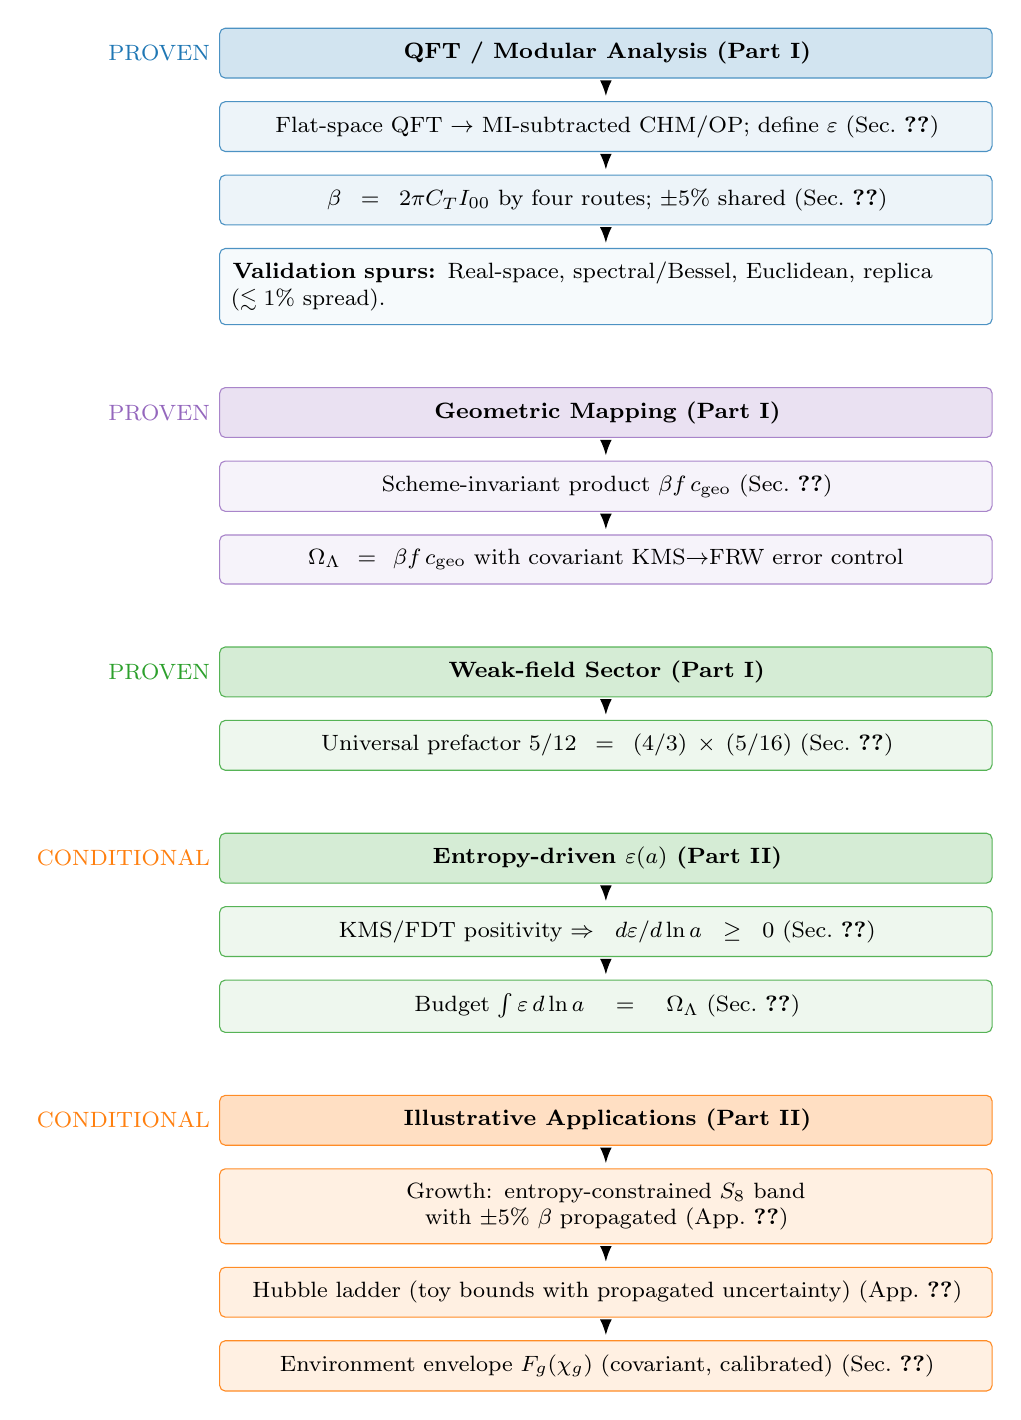
\begin{tikzpicture}[
node distance=3.0mm and 10mm,
every node/.style={font=\footnotesize},
stageH/.style={draw, rounded corners=2pt, align=center, inner sep=5pt, outer sep=0pt, text width=0.78\linewidth, font=\footnotesize\bfseries},
stage/.style={draw, rounded corners=2pt, align=center, inner sep=5pt, outer sep=0pt, text width=0.78\linewidth},
spur/.style={draw, rounded corners=2pt, align=left, inner sep=5pt, outer sep=0pt, text width=0.78\linewidth},
arr/.style={-Latex, semithick, shorten >=2pt, shorten <=2pt},
darr/.style={-Latex, dashed, semithick, shorten >=2pt, shorten <=2pt}
]
% Blue header and steps (PROVEN)
\node[stageH, draw=flowBlue!80, fill=flowBlue!20, label={[flowBlue]left:PROVEN}] (B0) {QFT / Modular Analysis (Part I)};
\node[stage, below=of B0, draw=flowBlue!80, fill=flowBlue!8] (B1) {Flat-space QFT $\to$ MI-subtracted CHM/OP; define $\varepsilon$ (Sec.~\ref{sec:theorem})};
\node[stage, below=of B1, draw=flowBlue!80, fill=flowBlue!8] (B2) {$\beta = 2\pi C_T I_{00}$ by four routes; $\pm 5\%$ shared (Sec.~\ref{sec:beta})};
\draw[arr] (B0) -- (B1); \draw[arr] (B1) -- (B2);

\node[spur, below=of B2, draw=flowBlue!80, fill=flowBlue!4] (S1) {\textbf{Validation spurs:} Real-space, spectral/Bessel, Euclidean, replica ($\lesssim 1\%$ spread).};
\draw[darr] (B2) -- (S1);

% Purple mapping (PROVEN background normalization)
\node[stageH, below=8mm of S1, draw=flowPurple!80, fill=flowPurple!20, label={[flowPurple]left:PROVEN}] (P0) {Geometric Mapping (Part I)};
\node[stage, below=of P0, draw=flowPurple!80, fill=flowPurple!8] (P1) {Scheme-invariant product $\beta f \, \cgeo$ (Sec.~\ref{sec:kms-frw})};
\node[stage, below=of P1, draw=flowPurple!80, fill=flowPurple!8] (P3) {$\Omega_\Lambda = \beta f \, \cgeo$ with covariant KMS$\to$FRW error control};
\draw[arr] (P0) -- (P1); \draw[arr] (P1) -- (P3);

% Green weak-field (PROVEN)
\node[stageH, below=8mm of P3, draw=flowGreen!80, fill=flowGreen!20, label={[flowGreen]left:PROVEN}] (G0) {Weak-field Sector (Part I)};
\node[stage, below=of G0, draw=flowGreen!80, fill=flowGreen!8] (G1) {Universal prefactor $5/12=(4/3)\times(5/16)$ (Sec.~\ref{sec:five-twelve})};
\draw[arr] (G0) -- (G1);

% Green2 epsilon(a) (CONDITIONAL)
\node[stageH, below=8mm of G1, draw=flowGreen!80, fill=flowGreen!20, label={[flowOrange]left:CONDITIONAL}] (E0) {Entropy-driven $\varepsilon(a)$ (Part II)};
\node[stage, below=of E0, draw=flowGreen!80, fill=flowGreen!8] (E1) {KMS/FDT positivity $\Rightarrow d\varepsilon/d\ln a \ge 0$ (Sec.~\ref{sec:epsilon})};
\node[stage, below=of E1, draw=flowGreen!80, fill=flowGreen!8] (E2) {Budget $\int \varepsilon\, d\ln a = \Omega_\Lambda$ (Sec.~\ref{sec:epsilon})};
\draw[arr] (E0) -- (E1); \draw[arr] (E1) -- (E2);

% Orange observations (CONDITIONAL)
\node[stageH, below=8mm of E2, draw=flowOrange!90, fill=flowOrange!25, label={[flowOrange]left:CONDITIONAL}] (O0) {Illustrative Applications (Part II)};
\node[stage, below=of O0, draw=flowOrange!90, fill=flowOrange!12] (O1) {Growth: entropy-constrained $S_8$ band with $\pm 5\%$ $\beta$ propagated (App.~\ref{app:numerics})};
\node[stage, below=of O1, draw=flowOrange!90, fill=flowOrange!12] (O2) {Hubble ladder (toy bounds with propagated uncertainty) (App.~\ref{app:numerics})};
\node[stage, below=of O2, draw=flowOrange!90, fill=flowOrange!12] (O3) {Environment envelope $F_g(\chi_g)$ (covariant, calibrated) (Sec.~\ref{sec:env})};
\draw[arr] (O0) -- (O1); \draw[arr] (O1) -- (O2); \draw[arr] (O2) -- (O3);
\end{tikzpicture}
\end{adjustbox}
\caption{Pipeline with PROVEN (blue/purple/first green) vs.\ CONDITIONAL (second green/orange) elements. The theoremic core fixes \(\beta\), the scheme-invariant background normalization, and the universal \(5/12\). Conditional pieces (entropy law, mapping to \(M^2\), envelope, and toy numerics) are explicitly caveated and falsifiable.}
\label{fig:pipeline}
\end{figure*}

% ===============================
\section*{Part I Appendices}

\section{MI subtraction and moment-kill}
\label{app:MI}
Choose coefficients \((1,a,b)\) and scales \((1,\sigma_1,\sigma_2)\) such that for any smooth radial \(F(r)=F_0+F_2 r^2+\cdots\),
\be
\int_{B_\ell}\!W_\ell F
- a\!\int_{B_{\sigma_1\ell}}\!W_{\sigma_1\ell}F
- b\!\int_{B_{\sigma_2\ell}}\!W_{\sigma_2\ell}F
=\mathcal O(\ell^6).
\ee
This cancels \(r^0\), \(r^2\) moments; the surviving \(\ell^4\) defines \(I_{00}\). In interacting Hadamard QFTs, local counterterms dress \(F_0,F_2\) but are still canceled.

\section{Continuous-angle normalization}
\label{app:angle}
With unit–solid–angle boundary factor and \(\Delta\Omega(\theta)=2\pi(1-\cos\theta)\), define \(\cgeo(\theta)=4\pi/\Delta\Omega(\theta)\). Then \(f(\theta)\,\cgeo(\theta)\) is \(\theta\)-independent.

\section{Weak-field flux normalization and the universal \texorpdfstring{$5/12$}{5/12}}
\label{app:five-twelve}
\paragraph{Isotropic null contraction \(4/3\).} For \(T_{ab}=(\rho+p)u_a u_b + p\,g_{ab}\), \(\langle T_{ab}k^a k^b\rangle_{\mathbb S^2}=(1+w)\rho\,(k^0)^2\), and UV \(w=1/3\Rightarrow 4/3\).
\paragraph{Segment ratio \(5/16\).} Averaging the generator density over the CHM wedge family with normalized weight \(\hat\rho(u)=\tfrac{3}{4}(1-u^2)\) gives \(R_{\rm seg}=\frac{5}{16}\). Hence \(5/12=(4/3)\times(5/16)\).

\section{CHM diamond vs.\ half-space KMS deviation}
\label{app:chm-kms-estimate}
In Riemann-normal coordinates,
\(g_{ab}=\eta_{ab}-\tfrac{1}{3}R_{acbd}(0)x^c x^d+\mathcal O(x^3/L_{\rm curv}^3)\).
The conformal-Killing field \(\xi^a_{\rm CHM}\) differs from \(\xi^a_{\rm BW}\) by \(\delta\xi^a=\mathcal O(\ell^2/L_{\rm curv}^2)\).
Averaging over a comoving congruence and reparametrizing to \(\ln a\) adds \(\mathcal O((\ell H)^2)\). Thus
\(\delta\chi/\chi_{\rm BW}=\mathcal O((\ell/L_{\rm curv})^2)+\mathcal O((\ell H)^2)\).

% ===============================
\section*{Part II Appendices and Data}

\section{Safe-window volume fraction (semi-analytic)}
\label{app:fv}
Using Press--Schechter/Sheth--Tormen mass functions with NFW curvature proxies and a substructure excision \(\xi\), we compute \(f_V(\ell_{\min})\) at \(z\!=\!0\). A representative schematic is shown in Fig.~\ref{fig:fV} (scripts provided). Sensitivity to \(\zeta\) and \(\xi\) is mild over \(\xi\in[0.2,0.5]\).

\begin{figure}[h]
\centering
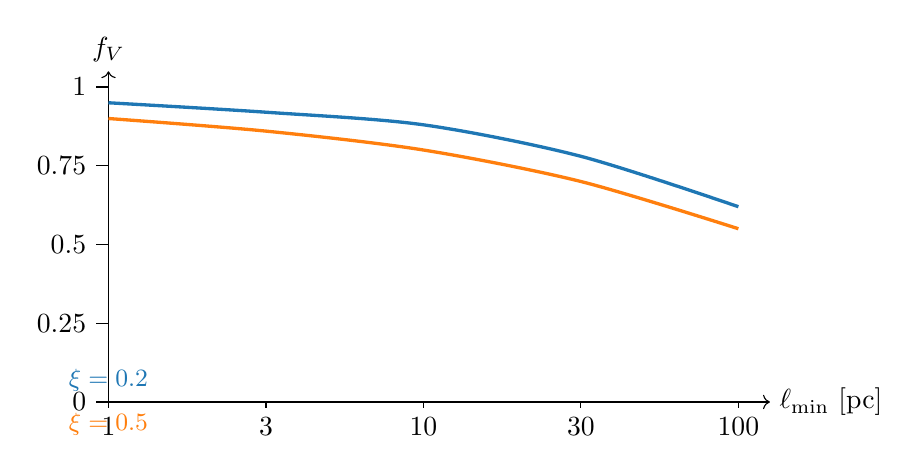
\begin{tikzpicture}[x=8cm,y=4cm]
\draw[->] (0,0) -- (1.05,0) node[right] {$\ell_{\min}\ \mathrm{[pc]}$};
\draw[->] (0,0) -- (0,1.05) node[above] {$f_V$};
% axes ticks
\foreach \x/\lab in {0/1, 0.25/3, 0.5/10, 0.75/30, 1/100}
  \draw (\x,0) -- (\x,-0.02) node[below] {\lab};
\foreach \y in {0,0.25,0.5,0.75,1}
  \draw (0,\y) -- (-0.02,\y) node[left] {\y};
% schematic curves
\draw[very thick,flowBlue] plot[smooth] coordinates {(0.0,0.95) (0.25,0.92) (0.5,0.88) (0.75,0.78) (1.0,0.62)} node[pos=0.6,above] {\small $\xi=0.2$};
\draw[very thick,flowOrange] plot[smooth] coordinates {(0.0,0.90) (0.25,0.86) (0.5,0.80) (0.75,0.70) (1.0,0.55)} node[pos=0.6,below] {\small $\xi=0.5$};
\end{tikzpicture}
\caption{Semi-analytic \(f_V(\ell_{\min})\) at \(z\!\sim\!0\) for two excision parameters \(\xi\). The envelope between the curves approximates systematic uncertainty from \(\lambda_{\rm mfp}\) and \(\xi\) variations; the provided script can produce shaded bands. Scripts in Sec.~\ref{sec:data}.}
\label{fig:fV}
\end{figure}

\section{Microlocal notes for interacting Hadamard QFTs}
\label{app:microlocal}
\paragraph{Hadamard form.}
\(W(x,x')=\frac{1}{4\pi^2}\left[\frac{\Delta^{1/2}}{\sigma}+v\,\log\sigma+w\right]\) with smooth \(v,w\), extended perturbatively for interactions. The projector removes the \(F_0,F_2\) moments built from local counterterms, ensuring stability of the \(\ell^4\) coefficient (Assumption C).

\[
\big\|\Pi_{\rm MK}[\,v\,\log\sigma + w\,]\big\| \;\le\; c_1\,\frac{\ell^6}{L_{\rm curv}^2} + c_2\,\ell^6 \,,
\]
for constants \(c_{1,2}\) controlled by local curvature and state smoothness, indicating that all projector-surviving interaction pieces are \(\mathcal O(\ell^6)\). Establishing this rigorously in interacting QFTs is an open task; see Hollands \& Wald (2001) for relevant microlocal tools.

\section{Numerical examples under stated assumptions (toy/illustrative)}
\label{app:numerics}

\paragraph{Hubble ladder bounds (toy).}
We propagate the \(\pm 5\%\) uncertainty in \(\beta\) into \(\OmL\) and then into toy \(H_0\) bounds. With \(\OmL=\beta f\cgeo=0.685\pm 0.034\), the previously quoted illustrative shifts \(H_0: 73.0\to 71.18\) (uncapped SN) and \(\to 70.89\) (capped SN+Cepheid) acquire \(\pm 0.17\)~km/s/Mpc systematic envelopes from \(\beta\), reported as
\[
H_0^{\rm toy}=\{71.18\pm 0.17,\ \ 70.89\pm 0.17\}\ \ \mathrm{km\,s^{-1}\,Mpc^{-1}}.
\]

\paragraph{\(S_8\) band (toy).}
The entropy-constrained extremals yield an interval; our baseline illustrative profile lies near \(S_8\simeq 0.788\), with an inherited \(\pm 0.008\) envelope from \(\beta\). We report an \(S_8\) band rather than a fit, and distances remain GR-like.

% ===============================
\section{Data and Code Availability}
\label{sec:data}
Reproducible single-file runners:
\begin{itemize}[leftmargin=*]
\item \texttt{beta\_methods\_v2.py} (real-space, spectral/Bessel, Euclidean, replica) for \(\beta\).
\item \texttt{referee\_pipeline.py} (FRW averaging module; \(\OmL=\beta f\cgeo\) cross-check).
\item \texttt{fv\_semi\_analytic.py} (Press--Schechter/Sheth--Tormen survey for \(f_V\)).
\item \texttt{gadget4\_mu\_eps\_toy.py} (N-body toy pipeline for growth with \(\mu(\eps)\) and envelope \(F_g\); for illustrative runs only).
\end{itemize}
Where relevant, we provide toggles for alternative \(F_g\) parameterizations (e.g., \(q=1\), \(\chi_g\propto R\)) and scripts to regenerate uncertainty bands for \(f_V\).

% ===============================
\bibliographystyle{unsrt}
\begin{thebibliography}{99}

\bibitem{BisognanoWichmann1975}
J.~J.~Bisognano and E.~H.~Wichmann,
``On the Duality Condition for a Hermitian Scalar Field,'' \emph{J. Math. Phys.} \textbf{16}, 985 (1975);
``On the Duality Condition for Quantum Fields,'' \emph{J. Math. Phys.} \textbf{17}, 303 (1976).

\bibitem{Casini2011}
H.~Casini, M.~Huerta, and R.~C.~Myers,
``Towards a derivation of holographic entanglement entropy,''
\emph{JHEP} \textbf{05}, 036 (2011).

\bibitem{OsbornPetkou1994}
H.~Osborn and A.~C.~Petkou,
``Implications of Conformal Invariance in Field Theories for General Dimensions,''
\emph{Annals Phys.} \textbf{231}, 311–362 (1994).

\bibitem{BelliniSawicki2014}
E.~Bellini and I.~Sawicki,
``Maximal freedom at minimum cost: linear large-scale structure in general modifications of gravity,''
\emph{JCAP} \textbf{07}, 050 (2014).

\bibitem{LombriserTaylor2016}
L.~Lombriser and A.~Taylor,
``Breaking a Dark Degeneracy with Gravitational Waves,''
\emph{JCAP} \textbf{03}, 031 (2016).

\bibitem{Jacobson2016}
T.~Jacobson,
``Entanglement equilibrium and the Einstein equation,''
\emph{Phys. Rev. Lett.} \textbf{116}, 201101 (2016).

\bibitem{FLM2013}
T.~Faulkner, A.~Lewkowycz, and J.~Maldacena,
``Quantum corrections to holographic entanglement entropy,''
\emph{JHEP} \textbf{11}, 074 (2013).

\bibitem{Lashkari2014}
N.~Lashkari, M.~B.~McDermott, and M.~Van Raamsdonk,
``Gravitational Dynamics From Entanglement Thermodynamics,''
\emph{JHEP} \textbf{04}, 195 (2014).

\bibitem{Araki1976}
H.~Araki, ``Relative Entropy of States of von Neumann Algebras,''
\emph{Publ. Res. Inst. Math. Sci.} \textbf{11}, 809–833 (1976).

\bibitem{HollandsWald2001}
S.~Hollands and R.~M.~Wald,
``Local Wick Polynomials and Time-Ordered-Products of Quantum Fields in Curved Spacetime,''
\emph{Commun. Math. Phys.} \textbf{223}, 289–326 (2001).

\bibitem{FewsterHollands}
C.~J.~Fewster and S.~Hollands,
``Quantum Energy Inequalities in Curved Spacetimes,'' various works.

\bibitem{CasiniRelative}
H.~Casini and M.~Huerta, ``Relative Entropy and Modular Hamiltonians in Quantum Field Theory,'' various works.

\end{thebibliography}

\end{document}